\documentclass[11pt]{article}

\usepackage[margin=1in]{geometry}
\usepackage[T1]{fontenc}
\usepackage{lmodern}
\usepackage{microtype}
\usepackage{amsmath}
\usepackage{graphicx}
\usepackage{booktabs}
\usepackage{multirow}
\usepackage{xcolor}
\usepackage{caption}
\usepackage{subcaption}
\usepackage{enumitem}
\usepackage{pifont}
\usepackage{tikz}
\usetikzlibrary{arrows.meta,positioning,shapes.geometric}
\usepackage[colorlinks=true,linkcolor=blue!50!black,citecolor=blue!50!black,urlcolor=blue!50!black]{hyperref}

\setlist{leftmargin=*,itemsep=2pt,topsep=3pt}
\newcommand{\fcfs}{\textsc{fcfs}}
\newcommand{\maxseqs}{\texttt{max\_num\_seqs}}

\title{Preempt Only When the Batch Is Full:\\
Saturation-Triggered MLFQ Scheduling for LLM Serving}
\author{Aaryan Pathak (124cs0065) \and Aniket Ware (524cs0012)}
\date{October 2026\\[4pt]
\small Code: \url{https://github.com/Neuro1729/vllm-os} (branch \texttt{mixed-batching})}

\begin{document}
\maketitle

\begin{abstract}
Continuous-batching LLM servers such as vLLM admit requests first-come-first-served until
\maxseqs{} requests are running; after that, a new request waits for a running one to finish,
whatever its priority (vLLM issue \#40004). Preemptive MLFQ schedulers such as FastServe fix
head-of-line blocking by re-ranking and preempting at every iteration, at the price of a much larger
KV-cache footprint and host-memory swapping. We observe that in a continuous-batching engine
preemption is only needed when the batch is full. Our scheduler behaves exactly like continuous
batching below saturation. Once the batch is full, it lets only fresh short requests evict a running
request, ranks requests by size so that no priorities are needed, and \emph{pauses} the victim with
its KV cache kept on the GPU. With vLLM-style mixed prefill/decode batching, on a nano-vllm based
engine, it cuts chat time-to-first-token p99 from 675\,ms to 37\,ms with a full batch, matches the
original scheduler's throughput within 0.1\%, and copies no KV cache.
\end{abstract}

%=====================================================================
\section{Introduction}
%=====================================================================

LLM servers increasingly mix latency-sensitive requests (chat, voice) with long background work
(coding agents). vLLM~\cite{vllm} serves them with continuous batching~\cite{orca}: requests join and
leave the batch at every iteration, up to \maxseqs{} at a time, in arrival order. When all
\maxseqs{} slots are held by long agent turns, a short interactive request has to wait for one of
them to finish, which can take seconds. Priority scheduling does not help, because the request is
already first in line; there is no free slot. This is vLLM issue \#40004~\cite{issue40004}.

\paragraph{Key idea.} Continuous batching already removes head-of-line blocking \emph{as long as the
batch has room}. We therefore keep it unchanged and add preemption only for the saturated case:
\begin{itemize}
  \item below saturation, nothing is ever preempted;
  \item at saturation, a fresh short request may evict the worst-ranked running request, where rank
    is the request's size (prompt plus generated tokens);
  \item the victim is paused with its KV cache left on the GPU instead of being swapped or recomputed;
  \item prefill and decode share each step (mixed batching), so admissions do not stall the batch.
\end{itemize}

\paragraph{Results.} On Qwen3-0.6B and one H100, with a full batch our scheduler matches strict
priority scheduling on chat latency even when no priorities are set, at the original scheduler's
throughput, and it never preempts when the batch is not full (\S\ref{sec:eval}).

%=====================================================================
\section{The Problem and Prior Work}
\label{sec:related}
%=====================================================================

\paragraph{vLLM issue \#40004.} In the V1 scheduler the waiting-request loop stops as soon as
\texttt{len(running) == max\_num\_running\_reqs}; preemption exists only for KV-cache
pressure~\cite{issue40004}. Users report a 6.8\,s wait for a priority-0 request with
\texttt{--max-num-seqs 8} and zero preemptions, and a voice-call p95 of 10.1\,s next to coding agents
against 1.8\,s alone~\cite{issue40004}. Several fix PRs (\#40087, \#45558, \#45561, \#54530,
\#63350/\#63351) add strict-priority preemption at \maxseqs{} or under KV pressure. As of October 2026
none is merged: \#40087 is marked stale and \#54530 needs a rebase and has no approving
review~\cite{pr40087,pr54530}. Review raised ping-pong between equal priorities, victims evicted for a
newcomer that still cannot be admitted, and LoRA accounting~\cite{issue40004,pr54530}. All of them
also require clients to set priorities.

\paragraph{FastServe.} FastServe~\cite{fastserve,fastserve-nsdi} introduced a skip-join MLFQ for LLM
inference (Figure~\ref{fig:fastserve}): a job joins the queue whose quantum covers its profiled
prefill time, is demoted when it uses up its quantum, and is promoted when starved. Every iteration
the scheduler runs the top \texttt{MaxBatchSize} jobs and preempts the rest. Keeping all preempted
jobs' caches costs up to $7\times$ the KV memory of \fcfs{}, so FastServe adds proactive KV swapping
to host memory and reserved KV slots~\cite{fastserve-nsdi}. It was motivated by serving systems
that ``use run-to-completion processing''~\cite{fastserve-nsdi}. In an engine that already has
continuous batching, a request that is not in a full batch blocks nobody, so most of this preemption
buys nothing.

\paragraph{Other attempts.} Fu et al.\ implemented an MLFQ ``in 1.2k lines of Python code'' on
vLLM v0.4.1 as a research baseline and note that it ``introduces substantial
complexity''~\cite{ltr}; it was not upstreamed. An open SGLang PR adds a skip-join MLFQ that avoids
preemption altogether~\cite{sglang45688}. We found no MLFQ PR, issue or RFC in vLLM itself.

\paragraph{Why it stayed open.} (1) Research MLFQs replace the scheduler instead of being a small
change to it. (2) Preemption is costly by default: vLLM V1 recomputes victims~\cite{vllm-opt}, and
frequent preemption can lose more throughput than it saves latency. (3) Priority-based fixes only
help clients that tag requests. (4) The problem appears only when long requests fill \maxseqs{},
which common benchmarks rarely do.

\begin{figure}[t]
\centering
\begin{subfigure}[t]{0.49\linewidth}
\centering
\resizebox{\linewidth}{!}{%
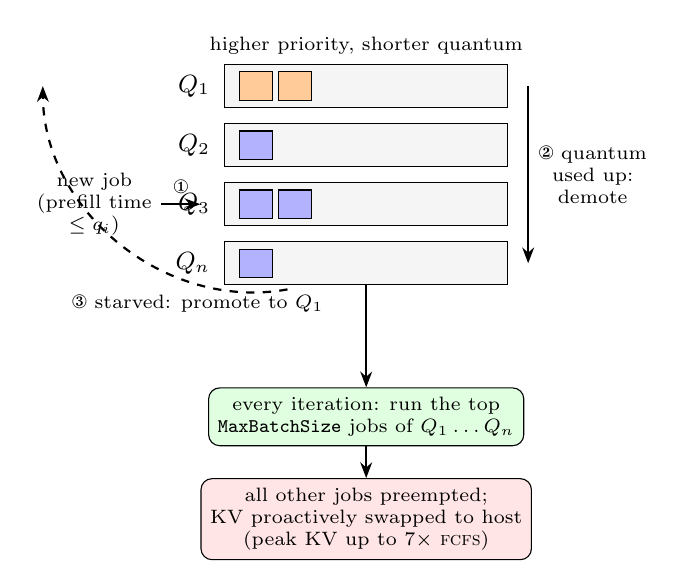
\begin{tikzpicture}[
  q/.style={draw, minimum width=3.6cm, minimum height=0.55cm, fill=gray!8},
  job/.style={draw, fill=#1, minimum width=0.42cm, minimum height=0.36cm, inner sep=0pt},
  ar/.style={-{Stealth[length=2mm]}, thick},
  lb/.style={font=\scriptsize, align=center}]
\foreach \i/\n in {0/1,1/2,2/3,3/n} {
  \node[q] (Q\n) at (0,-0.75*\i) {};
  \node[font=\small, anchor=east] at (Q\n.west) {$Q_{\n}$\,};
}
\node[font=\scriptsize, anchor=south] at (Q1.north) {higher priority, shorter quantum};
\node[job=orange!40] at ([xshift=-1.4cm]Q1.center) {};
\node[job=orange!40] at ([xshift=-0.9cm]Q1.center) {};
\node[job=blue!30]   at ([xshift=-1.4cm]Q2.center) {};
\node[job=blue!30]   at ([xshift=-1.4cm]Q3.center) {};
\node[job=blue!30]   at ([xshift=-0.9cm]Q3.center) {};
\node[job=blue!30]   at ([xshift=-1.4cm]Qn.center) {};
\node[lb, anchor=east] (arr) at (-2.6,-1.5) {new job\\(prefill time\\$\le q_i$)};
\draw[ar] (arr.east) -- node[lb, above, sloped] {\ding{172}} ([xshift=-0.3cm]Q3.west);
\draw[ar] ([xshift=0.25cm]Q1.east) -- node[lb, right] {\ding{173} quantum\\used up:\\demote} ([xshift=0.25cm]Qn.east);
\draw[ar, dashed] ([xshift=-1.0cm, yshift=-0.05cm]Qn.south) to[bend left=50] node[lb, below, pos=0.25] {\ding{174} starved: promote to $Q_1$} ([xshift=-2.3cm]Q1.west);
\node[draw, rounded corners, fill=green!12, lb, minimum width=3.6cm] (batch) at (0,-4.2) {every iteration: run the top\\\texttt{MaxBatchSize} jobs of $Q_1 \ldots Q_n$};
\draw[ar] (Qn.south) -- (batch.north);
\node[draw, rounded corners, fill=red!10, lb, minimum width=3.6cm] (host) at (0,-5.5) {all other jobs preempted;\\KV proactively swapped to host\\(peak KV up to $7\times$ \textsc{fcfs})};
\draw[ar] (batch.south) -- (host.north);
\end{tikzpicture}}
\caption{FastServe's skip-join MLFQ, adapted from~\cite{fastserve-nsdi} (Fig.~6, Alg.~1).}
\label{fig:fastserve}
\end{subfigure}\hfill
\begin{subfigure}[t]{0.49\linewidth}
\centering
\resizebox{\linewidth}{!}{%
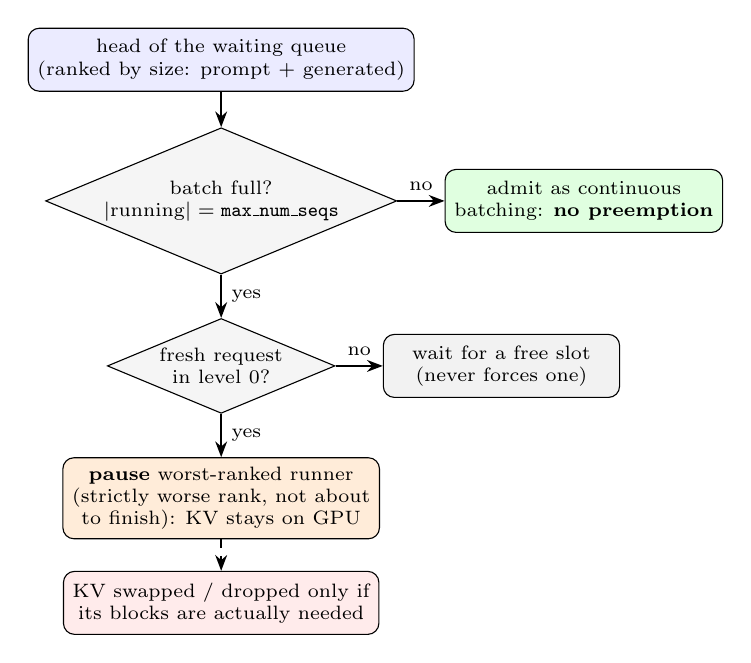
\begin{tikzpicture}[
  dec/.style={draw, diamond, aspect=2.4, fill=gray!8, font=\scriptsize, align=center, inner sep=1pt},
  box/.style={draw, rounded corners, font=\scriptsize, align=center, minimum width=3.0cm, minimum height=0.8cm},
  ar/.style={-{Stealth[length=2mm]}, thick},
  lb/.style={font=\scriptsize}]
\node[box, fill=blue!8] (new) at (0,0) {head of the waiting queue\\(ranked by size: prompt + generated)};
\node[dec, below=0.45cm of new] (full) {batch full?\\$|\text{running}| = \maxseqs$};
\node[box, fill=green!12, right=0.6cm of full] (cb) {admit as continuous\\batching: \textbf{no preemption}};
\node[dec, below=0.55cm of full] (fresh) {fresh request\\in level 0?};
\node[box, fill=gray!10, right=0.6cm of fresh] (wait) {wait for a free slot\\(never forces one)};
\node[box, fill=orange!15, below=0.55cm of fresh] (pause) {\textbf{pause} worst-ranked runner\\(strictly worse rank, not about\\to finish): KV stays on GPU};
\node[box, fill=red!8, below=0.4cm of pause] (lazy) {KV swapped / dropped only if\\its blocks are actually needed};
\draw[ar] (new) -- (full);
\draw[ar] (full) -- node[lb, above] {no} (cb);
\draw[ar] (full) -- node[lb, right] {yes} (fresh);
\draw[ar] (fresh) -- node[lb, above] {no} (wait);
\draw[ar] (fresh) -- node[lb, right] {yes} (pause);
\draw[ar, dashed] (pause) -- (lazy);
\end{tikzpicture}}
\caption{Our saturation-triggered MLFQ.}
\label{fig:ours}
\end{subfigure}
\caption{Where preemption happens. FastServe re-ranks and preempts at every iteration and offloads
the caches of preempted jobs to host memory. We leave continuous batching untouched until the batch
is full, then let only a fresh short request pause one runner, without copying its KV cache.}
\label{fig:fastserve-vs-ours}
\end{figure}

%=====================================================================
\section{Design}
\label{sec:design}
%=====================================================================

\paragraph{Two regimes.} Below saturation ($|\text{running}| < \maxseqs$) the scheduler is
continuous batching: waiting requests are admitted best rank first while KV blocks are free, and a
request that does not fit in the KV cache waits, as in \fcfs{}. At saturation the head of the waiting
queue may evict running requests under the rules below (Figure~\ref{fig:ours}). Running out of KV
during decode preempts as in vLLM, but takes the worst-ranked victim.

\paragraph{Size-based levels.} With level boundaries $b_0 < b_1 < \dots$ in tokens (default
1\,024/4\,096/8\,192), a request with $s$ tokens is in level $\min\{i : s \le b_i\}$. Rank is
$(\text{level}, \text{priority})$, so priorities only break ties. A long prompt starts low (a token
version of FastServe's skip-join) and a request is demoted as it generates. A waiting request is
promoted one level every \texttt{aging\_steps} steps and then gets that level's whole band again.
A short chat thus outranks a long agent context without anyone saying so.

\paragraph{Who may evict whom.} A waiting request may evict only if it has never been preempted and
is in level 0. The victim must rank strictly worse (equal ranks never evict each other), must have
run at least \texttt{min\_resident\_steps} steps, and must have at least 16 tokens left before its
\texttt{max\_tokens}. Eviction is all-or-nothing: nobody is evicted for a request that would still not
fit. The fresh-and-short rule matters: if any better-ranked request may evict, 44\% of preemptions
are agents evicting agents (a new agent turn at a higher level, or an aged-up victim), which costs a
KV copy and buys no latency.

\paragraph{Pause instead of swap.} When the batch is full, the scarce resource is the slot, not KV
memory. A victim evicted only for its slot is \emph{paused}: it leaves the batch but keeps its KV
blocks on the GPU and resumes with no copy and no recompute. Its blocks are swapped to host memory or
dropped for recompute only if a newcomer, a decode step or a swap-in actually needs them, and idle
paused blocks are reclaimed before any running request is evicted.

\paragraph{No waiting, low overhead.} With pausing an eviction is cheap, so a newcomer evicts
immediately instead of waiting for a slot to free up; churn is bounded by
\texttt{min\_resident\_steps}. The waiting queue is re-sorted only when its order can change, and
aging uses a global step counter, so a scheduler step costs 15\,$\mu$s with 500 waiting requests
instead of 109\,$\mu$s for re-sorting and aging the whole queue (\fcfs{}: 5\,$\mu$s).

\paragraph{Mixed batching.} nano-vllm~\cite{nanovllm} runs each step either as a prefill or as a
decode, so every admission stalls the whole batch. As in vLLM V1 and
Sarathi-Serve~\cite{sarathi,vllm-opt}, we reserve one token per running request in each step and
fill the rest of the token budget with (chunked) prefills. Mixed steps reuse the variable-length
prefill path, a decode being a one-token query over its paged cache; pure decode steps still use
CUDA graphs.

\paragraph{Footprint.} Everything is opt-in. With the default \fcfs{} policy and mixed batching off,
the scheduler's decisions are unchanged. The whole change is about 485 lines over nano-vllm.

%=====================================================================
\section{Evaluation}
\label{sec:eval}
%=====================================================================

\paragraph{Setup.} One NVIDIA H100 PCIe, Qwen3-0.6B (bf16), CUDA graphs, 256-token KV blocks.
\emph{Agents} are closed-loop multi-turn sessions (300--600-token start, 128--384 tokens per turn, a
50--150-token tool result appended, 0.5\,s think time, priority 1). \emph{Chat} arrives as a Poisson
stream (32--128-token prompts, 16--128 output tokens, priority 0). Each run has 45\,s of arrivals;
results are means over three seeds. MLFQ levels are 256/512/1\,024 tokens. Scenarios:
\emph{batch-cap} (8 slots, 12 agents, 4 chats/s, ample KV: the \#40004 case), \emph{no-priority}
(the same with equal priorities), \emph{kv-pressure} (64 slots, 10k tokens of KV), \emph{normal}
(32 slots, 4 agents, 1 chat/s) and \emph{all-short} (chat only, 40/s into 8 slots). \fcfs{} is
nano-vllm's original scheduler; \emph{priority + swap} is strict priority with preemption at
\maxseqs{} and swapped victims, i.e.\ what the \#40004 PRs add; \emph{ours} is the
saturation-triggered MLFQ of \S\ref{sec:design} with mixed batching.

\begin{table}[t]
\centering
\small
\caption{Results, mean of three seeds. Throughput is relative to \fcfs{} in the same scenario.}
\label{tab:main}
\begin{tabular}{llrrrrr}
\toprule
scenario & scheduler & TTFT p50 & TTFT p99 & agent e2e p50 & tok/s & vs \fcfs{} \\
\midrule
\multirow{3}{*}{batch-cap}
 & \fcfs{}          & 280\,ms & 675\,ms & 1.25\,s & 1935 & --- \\
 & priority + swap  & 25\,ms  & 42\,ms  & 1.28\,s & 1860 & $-3.9$\% \\
 & ours             & \textbf{23\,ms} & \textbf{37\,ms} & 1.19\,s & 1933 & $-0.1$\% \\
\midrule
\multirow{3}{*}{no-priority}
 & \fcfs{}          & 257\,ms & 562\,ms & 1.23\,s & 1924 & --- \\
 & priority + swap  & 283\,ms & 665\,ms & 1.24\,s & 1907 & $-0.9$\% \\
 & ours             & \textbf{24\,ms} & \textbf{39\,ms} & 1.19\,s & 1923 & $-0.1$\% \\
\midrule
\multirow{3}{*}{kv-pressure}
 & \fcfs{}          & 270\,ms & 1101\,ms & 1.30\,s & 1848 & --- \\
 & priority + swap  & 28\,ms  & 146\,ms  & 1.38\,s & 1789 & $-3.2$\% \\
 & ours             & \textbf{28\,ms} & \textbf{143\,ms} & 1.28\,s & 1834 & $-0.8$\% \\
\midrule
\multirow{2}{*}{normal}
 & \fcfs{}          & 29\,ms & 34\,ms & 0.79\,s & 836 & --- \\
 & ours             & 30\,ms & 40\,ms & 0.81\,s & 836 & $+0.1$\% \\
\midrule
\multirow{2}{*}{all-short}
 & \fcfs{}          & 10.7\,s & 20.8\,s & --- & 1482 & --- \\
 & ours             & 9.2\,s  & 17.9\,s & --- & 1554 & $+4.8$\% \\
\bottomrule
\end{tabular}
\end{table}

\paragraph{Full batch.} With every slot taken by agents (Figure~\ref{fig:results}), our scheduler
lowers chat TTFT p99 from 675\,ms to 37\,ms (18$\times$) when chat has priority and from 562\,ms to
39\,ms (14$\times$) when nobody sets priorities. Priority + swap reaches similar latency only when
priorities are set (42\,ms) and does nothing without them (665\,ms); it also loses 3.9\% throughput
and copies about 135 KV caches to host memory per run. Ours stays within 0.1\% of \fcfs{}'s
throughput, makes agent turns 3--5\% faster, and copies nothing: all of its roughly 125 preemptions
per run are pauses.

\paragraph{No saturation.} Under normal load and with only short requests our scheduler never
preempts (zero preemptions in every run) and matches \fcfs{}'s throughput under normal load
(Figure~\ref{fig:normal}). The 4.8\% gain with only short requests comes from mixed batching, which
gives \fcfs{} the same gain.

\paragraph{KV pressure.} With free slots there is no admission preemption; ordering by size and
choosing the largest victim when decode runs out of blocks lowers chat TTFT p99 from 1\,101\,ms to
143\,ms at 0.8\% throughput. Here evictions do need their blocks, so they are swapped.

\begin{figure}[t]
\centering
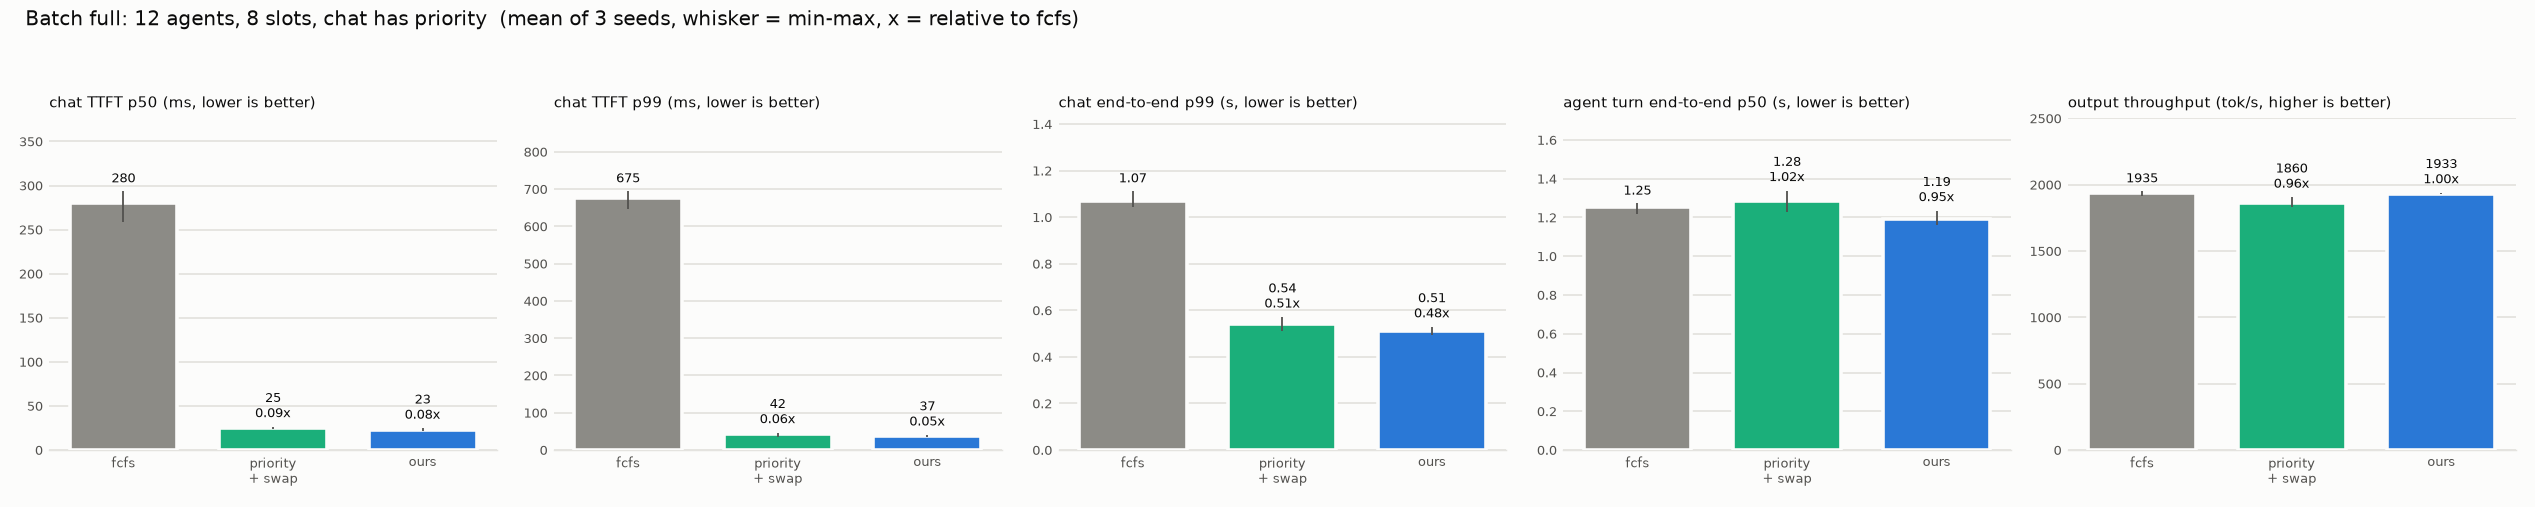
\includegraphics[width=\linewidth]{figures/results-batch-cap.png}\\[4pt]
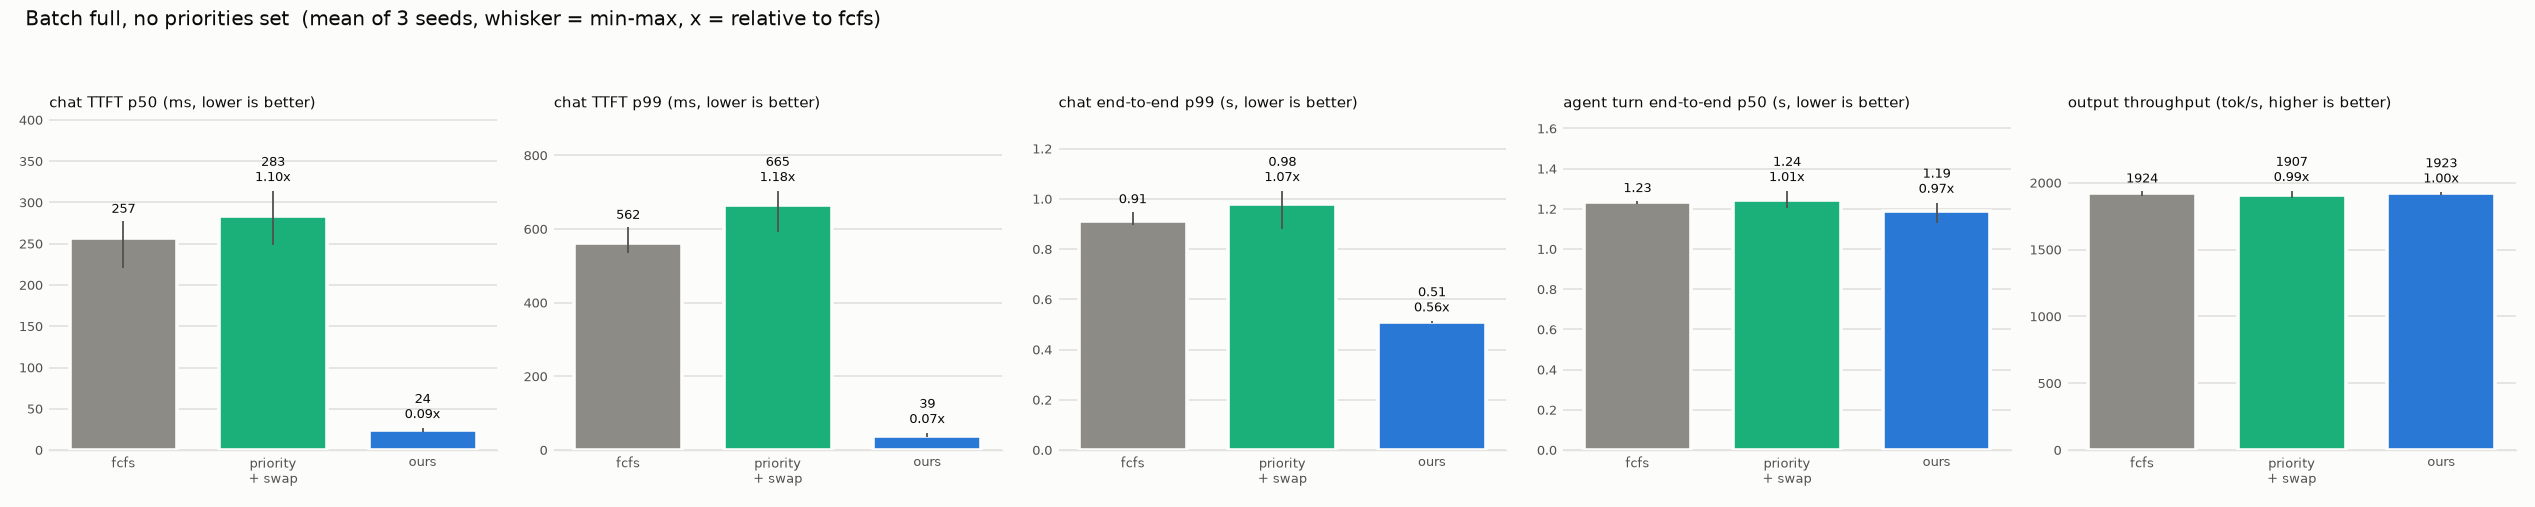
\includegraphics[width=\linewidth]{figures/results-no-priority.png}
\caption{Full batch, with priorities (top) and without (bottom). Mean of three seeds, whiskers
min--max, factors relative to \fcfs{}.}
\label{fig:results}
\end{figure}

\begin{figure}[t]
\centering
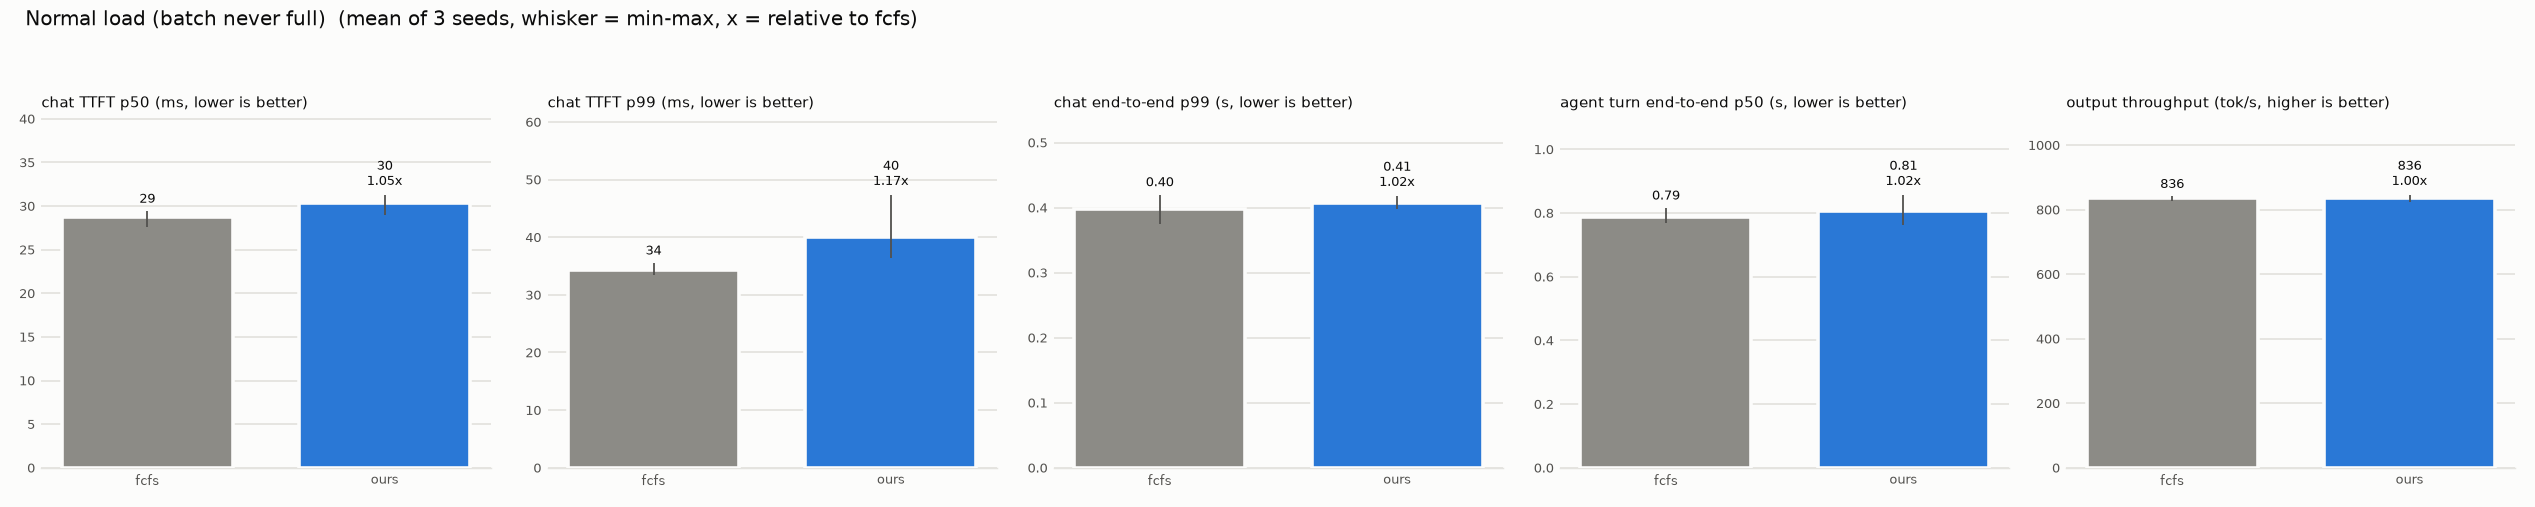
\includegraphics[width=\linewidth]{figures/results-normal.png}
\caption{Normal load: the batch never fills, our scheduler never preempts and behaves like \fcfs{}.}
\label{fig:normal}
\end{figure}

\paragraph{Limitations.} One small model on one GPU, a synthetic workload, 45\,s runs and three
seeds (single runs vary by about $\pm2$--$3\%$). Mixed batching also speeds up \fcfs{} itself
(+3\% with a full batch); against that stronger baseline our scheduler is about 3\% lower in
throughput, which we see as the inherent trade of giving slots to short requests. Porting to vLLM
needs the size-based rank, the eviction rules and a paused state at the \maxseqs{} check that the
\#40004 PRs patch, plus handling of LoRA, speculative decoding and pipeline parallelism, which our
prototype does not cover.

%=====================================================================
\section{Conclusion}
%=====================================================================

Head-of-line blocking in a continuous-batching LLM server is a saturation problem. Preempting only
when the batch is full, ranking requests by size, letting only fresh short requests evict and pausing
victims instead of copying their KV cache removes the blocking reported in vLLM issue \#40004 while
leaving normal operation untouched; with mixed batching it costs no measurable throughput.

%=====================================================================
\begin{thebibliography}{99}
\small

\bibitem{orca}
G.-I. Yu, J.~S. Jeong, G.-W. Kim, S.~Kim, and B.-G. Chun.
\newblock Orca: A distributed serving system for transformer-based generative models.
\newblock In \emph{OSDI}, 2022.

\bibitem{vllm}
W.~Kwon, Z.~Li, S.~Zhuang, Y.~Sheng, L.~Zheng, C.~H. Yu, J.~E. Gonzalez, H.~Zhang, and I.~Stoica.
\newblock Efficient memory management for large language model serving with PagedAttention.
\newblock In \emph{SOSP}, 2023.

\bibitem{sarathi}
A.~Agrawal, N.~Kedia, A.~Panwar, J.~Mohan, N.~Kwatra, B.~S. Gulavani, A.~Tumanov, and R.~Ramjee.
\newblock Taming throughput-latency tradeoff in LLM inference with Sarathi-Serve.
\newblock In \emph{OSDI}, 2024.

\bibitem{fastserve}
B.~Wu, Y.~Zhong, Z.~Zhang, S.~Liu, F.~Liu, Y.~Sun, G.~Huang, X.~Liu, and X.~Jin.
\newblock Fast distributed inference serving for large language models.
\newblock arXiv:2305.05920, 2023.

\bibitem{fastserve-nsdi}
B.~Wu, Y.~Zhong, Z.~Zhang, S.~Liu, F.~Liu, Y.~Sun, G.~Huang, X.~Liu, and X.~Jin.
\newblock FastServe: Iteration-level preemptive scheduling for large language model inference.
\newblock In \emph{NSDI}, 2026 (pre-publication version).

\bibitem{ltr}
Y.~Fu, S.~Zhu, R.~Su, A.~Qiao, I.~Stoica, and H.~Zhang.
\newblock Efficient LLM scheduling by learning to rank.
\newblock In \emph{NeurIPS}, 2024.

\bibitem{nanovllm}
nano-vllm. \url{https://github.com/GeeeekExplorer/nano-vllm}.

\bibitem{issue40004}
vLLM issue \#40004: Priority scheduling supports preemption of requests in the running queue by
requests in the waiting queue. \url{https://github.com/vllm-project/vllm/issues/40004}.

\bibitem{pr40087}
vLLM pull request \#40087. \url{https://github.com/vllm-project/vllm/pull/40087}.

\bibitem{pr54530}
vLLM pull request \#54530. \url{https://github.com/vllm-project/vllm/pull/54530}.

\bibitem{sglang45688}
SGLang pull request \#45688: skip-join MLFQ policy.
\url{https://github.com/sgl-project/sglang/pull/45688}.

\bibitem{vllm-opt}
vLLM documentation: Optimization and tuning.
\url{https://docs.vllm.ai/en/latest/configuration/optimization/}.

\end{thebibliography}

\end{document}
